\documentclass[dvisvgm,tikz]{standalone}

\usepackage[sfdefault]{inter}
\usetikzlibrary{shapes.geometric, arrows.meta, positioning, calc, fit, decorations.pathmorphing}

%%%%%%%%%%%%%%%%%%%%%%%%%%%%%%%%%%%%%%%%%%%%%%%%%%%
%Colors
% Warm gray to turquoise
\definecolor{warm_gray}{RGB}{128, 120, 115}
\definecolor{sage_gray}{RGB}{110, 125, 120}
\definecolor{pewter}{RGB}{91, 112, 114}
\definecolor{slate_blue}{RGB}{72, 107, 115}
\definecolor{steel_teal}{RGB}{53, 118, 125}
\definecolor{teal}{RGB}{27, 136, 140}
\definecolor{deep_aqua}{RGB}{15, 152, 155}
\definecolor{peacock_blue}{RGB}{0, 167, 171}
\definecolor{blue_green}{RGB}{0, 181, 185}
\definecolor{turquoise}{RGB}{0, 195, 200}

\definecolor{mygray}{gray}{0.9}

% Match our established color scheme
\definecolor{atoken}{RGB}{255, 152, 0}        % Orange for A token
\definecolor{gtoken}{RGB}{76, 175, 80}        % Green for G token
\definecolor{mainblue}{RGB}{74, 144, 226}     % Blue for A classes
\definecolor{maingreen}{RGB}{102, 187, 106}   % Light green for G classes
\definecolor{timegray}{RGB}{158, 158, 158}    % Gray for time component
%%%%%%%%%%%%%%%%%%%%%%%%%%%%%%%%%%%%%%%%%%%%%%%%%%%

\def \G {\textbf{G}}
\def \A {\textbf{A}}
\def \Q {\textbf{Q}}
\def \C {\textbf{C}}
\def \CC {\textbf{C*}}
\def \KA {\textbf{KLIMA}}
\def \KG {\textbf{KlimaX}}

\def \AG {$\overline{\textbf{AG}}$}
\def \AQ {$\overline{\textbf{AQ}}$}

\begin{document}
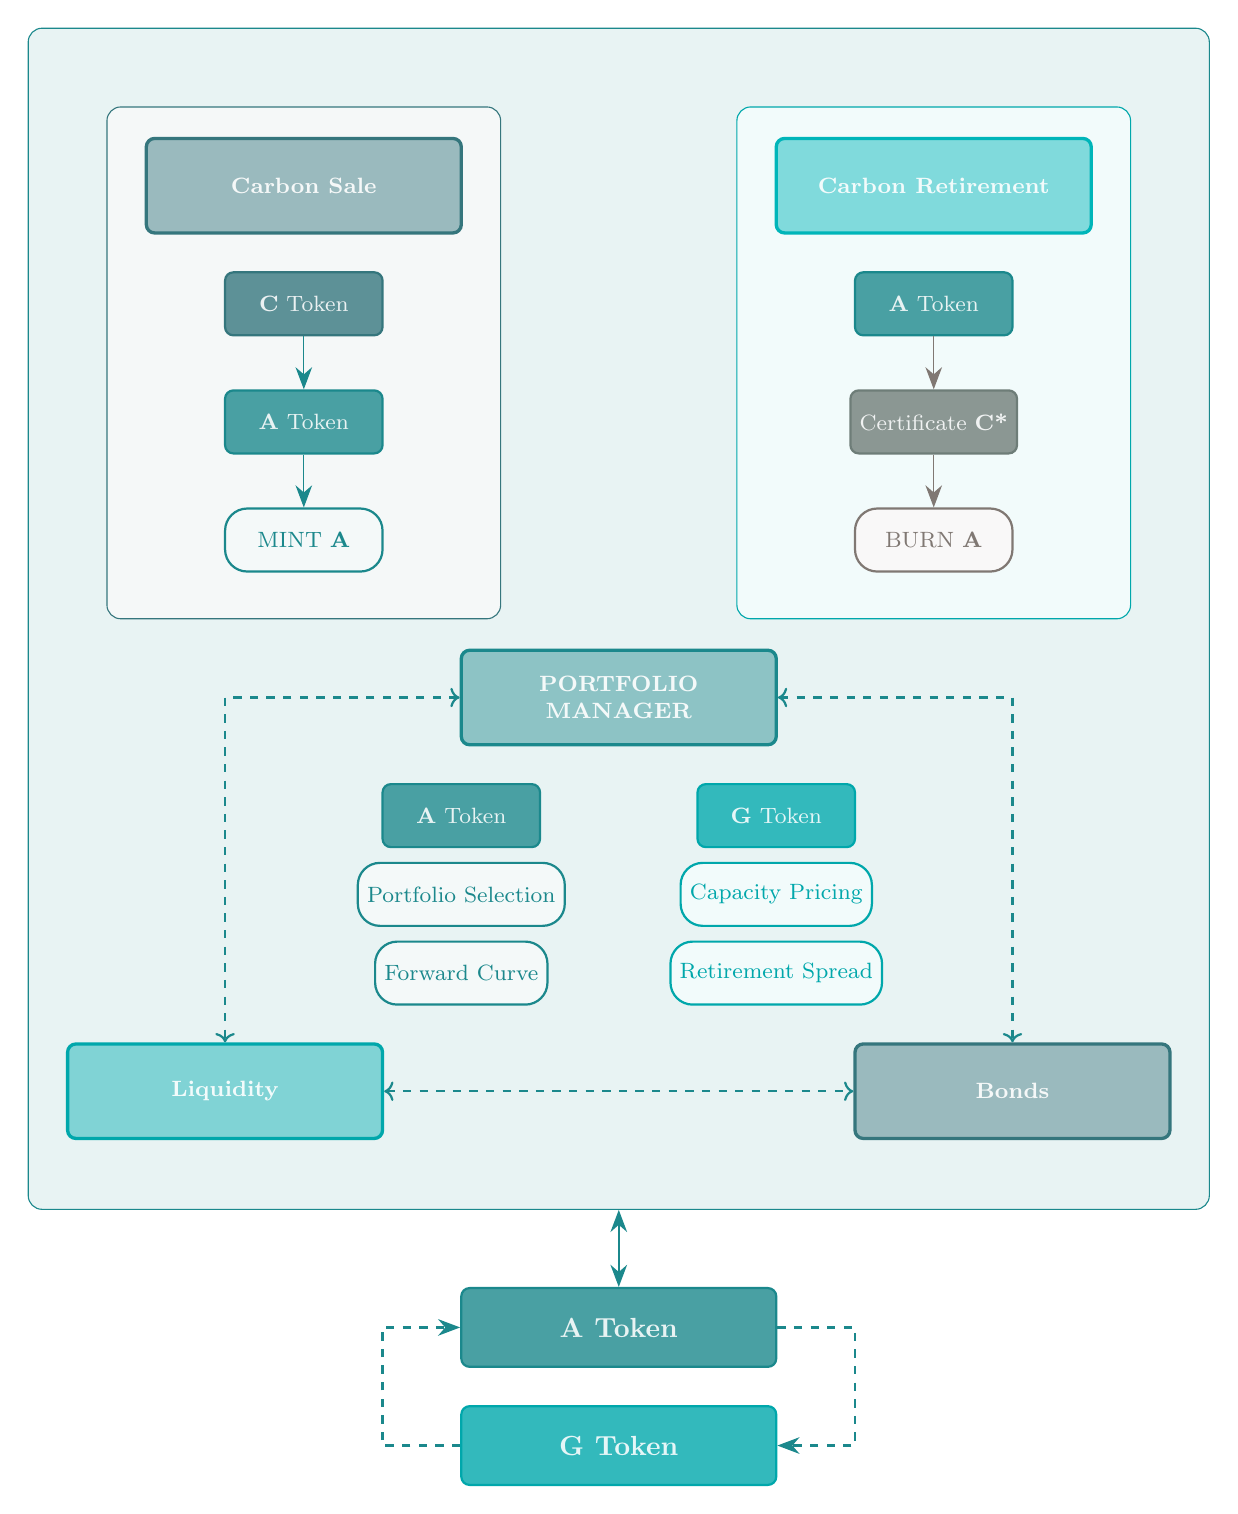
\begin{tikzpicture}[
    action/.style={
        rectangle,
        draw=#1,
        fill=#1!20,
        minimum width=2cm,
        minimum height=0.8cm,
        thick,
        rounded corners=3pt,
        text=#1,
        font=\footnotesize,
        align=center
    },
    token/.style={
        rectangle,
        draw=#1,
        fill=#1!80,
        minimum width=2cm,
        minimum height=0.8cm,
        thick,
        text=#1!10,
        rounded corners=3pt,
        font=\footnotesize,
        align=center
    },
    token_bg/.style={
        rectangle,
        draw=#1,
        fill=#1!80,
        minimum width=4cm,
        minimum height=1cm,
        thick,
        text=#1!10,
        rounded corners=3pt,
        font=\normalsize \bfseries,
        align=center
    },
    activity/.style ={
        rectangle,
        draw=#1,
        fill=#1!05,
        minimum width=2cm,
        minimum height=0.8cm,
        thick,
        rounded corners=8pt,
        text=#1,
        font=\footnotesize,
        align=center
    },
    title/.style={
        rectangle,
        draw=#1,thick,
        fill=#1!80,
        rounded corners=5pt,
        minimum width=2.8cm,
        minimum height=1.0cm,
        thick,
        text=white,
        font=\footnotesize\bfseries,
        align=center
    },
    market/.style={
        rectangle,
        draw=#1,very thick,
        fill=#1!50,
        text=#1!05,
        minimum width=4cm,
        minimum height=1.2cm,
        align=center,
        rounded corners=3pt, font=\footnotesize\bfseries
    },
    flow/.style={
        thick,
        #1
    },
    market_flow/.style={
        {Stealth[length=8pt]}-{Stealth[length=8pt]},
        thick,
        #1
    },
    arrow/.style={
        -{Stealth[length=8pt]},
        thin,
        #1
    },
    dash_arrow/.style={
        -{Stealth[length=8pt]},
        thick,
        #1, dashed, <->
    },
    dash_arrow_1/.style={
        -{Stealth[length=8pt]},
        thick,
        #1, dashed
    },
    column/.style={
        rectangle,
        draw=#1,
        fill=#1!05,
        minimum width=5cm,
        minimum height=6.5cm,
        rounded corners=5pt
    },
    column_bg/.style={
        rectangle,
        draw=#1,
        fill=#1!10,
        minimum width=15cm,
        minimum height=15cm,
        rounded corners=5pt
    },
]
\node[column_bg=teal] (col_bg) at (0,3) {};

\node[column=steel_teal] at (-4,6.25) {};
\node[column=peacock_blue] at (4,6.25) {};

\node[market=steel_teal] (sales) at (-4,8.5) {Carbon Sale};

\node[token=steel_teal] (carbon1) at (-4,7) {\C{} Token};
\node[token=teal] (token1) at (-4,5.5) {\A{} Token};

\node[activity=teal] (mint) at (-4,4) {MINT \A{}};

\node[market=blue_green] (retire) at (4,8.5) {Carbon Retirement};

\node[token=teal] (token2) at (4,7) {\A{} Token};


\node[token=sage_gray] (offset) at (4,5.5) {Certificate \CC{}};
\node[activity=warm_gray] (burn) at (4,4) {BURN \A{}};

\node[market=teal] (aam) at (0,2) {PORTFOLIO \\ MANAGER};

\node[token=teal] (atoken) at (-2,0.5) {\A{} Token};

\node[token=peacock_blue] (gtoken) at (2,0.5) {\G{} Token};

\node[activity=teal] (Portfolio) at (-2,-0.5) {Portfolio Selection};
\node[activity=teal] (forward) at (-2,-1.5) {Forward Curve};


\node[activity=peacock_blue] (capacity) at (2,-0.5) {Capacity Pricing};
\node[activity=peacock_blue] (spread) at (2,-1.5) {Retirement Spread};

\node[market=peacock_blue] (liquidity) at (-5,-3) {Liquidity};
\node[market=steel_teal] (bondmarket) at (5,-3) {Bonds};

\node[token_bg=teal] (big_a) at (0,-6) {\A{} Token};
\node[token_bg=peacock_blue] (big_g) at (0,-7.5) {\G{} Token};

% Token swap arrows
\draw[arrow=teal] (carbon1) -- (token1);

\draw[arrow=teal] (token1) -- (mint);

\draw[arrow=warm_gray] (token2) -- (offset);
\draw[arrow=warm_gray] (offset) -- (burn);


% Straight market connection arrows 
\draw[dash_arrow=teal] (aam.west) -| (liquidity.north);
\draw[dash_arrow=teal] (aam.east) -| (bondmarket.north);
\draw[dash_arrow=teal] (liquidity.east) -- (bondmarket.west);


\draw[market_flow=teal] (col_bg.south) -- (big_a.north);

\draw[dash_arrow_1=teal] (big_g.west) -- (-3,-7.5) -- (-3,-6) -- (big_a.west);

\draw[dash_arrow_1=teal] (big_a.east) -- (3,-6) -- (3,-7.5) -- (big_g.east);

\end{tikzpicture}
\end{document}
